\section{Study 2: long-horizon degradation under calibrated difficulty}
\label{sec:study2}

\subsection{The CDR-Stream benchmark}

Study 1 tasks span at most nine turns, and their difficulty is not controlled.
To study long horizons, we built CDR-Stream. It consists of 100-turn dialogues
in four domains:
\begin{itemize}
  \item a budget ledger;
  \item inventory logistics;
  \item a laboratory protocol;
  \item milestone chains.
\end{itemize}
Every user turn updates a shared state, for example a delivery, a correction or
a transfer, and asks one question about it. Exact solvers compute the gold
answer of every turn, so accuracy is observable at every turn.

Questions are drawn from six families: sum, difference, count-above-threshold,
maximum, what-if and share. Difficulty follows a 12-level ladder that changes one
complexity axis per step.

\paragraph{Calibrated difficulty.}
Before any stream was generated, a single-turn calibration stage mapped easy,
medium and hard regimes to ladder levels separately for each model and domain.
Its target bands were:
\begin{itemize}
  \item easy: 0.75--0.92;
  \item medium: 0.60--0.78;
  \item hard: 0.35--0.65.
\end{itemize}
The frozen fitting rule used isotonic regression and a one-sided trend test, and
it excluded domains that showed a ceiling, a floor or no trend.
Table~\ref{tab:s2map} lists the resulting mappings.

\paragraph{Scenarios.}
Each regime is a mixture: 50\% of turns at the centre level, 20\% at each
neighbour and 10\% from an adjacent regime. No scenario therefore consists of a
single question type or difficulty. The core scenarios are:
\begin{itemize}
  \item stationary easy (S0-E) and stationary hard (S0-H);
  \item a graded staircase, easy$\to$medium$\to$hard at turns 34 and 68 (S1);
  \item a sudden shift, easy$\to$hard at turn 51 (S2);
  \item a shift with recovery, easy$\to$hard$\to$easy at turns 34 and 67 (S3).
\end{itemize}

\paragraph{Models.}
The models were GPT-4o-mini, Llama-3 70B and Gemma 3 12B. They were chosen
because they passed the calibration rule and a technical pilot, not because of
any stream outcome.

Several other candidates were replaced before the main run:
\begin{itemize}
  \item Mistral-7B was at the accuracy floor;
  \item a larger Gemma model hit the ceiling;
  \item all Llama-4 variants produced near-identical repeated samples.
\end{itemize}
These replacements, and two recorded deviations for Llama-3 70B, are documented
in the supplementary material.

\begin{table}[t]
\centering
\caption{Study 2 frozen difficulty mappings (ladder levels for easy/medium/hard)
by model and domain. A dash marks a domain excluded by the calibration rule.}
\label{tab:s2map}
\small
\begin{tabular}{lcccc}
\toprule
Model & Budget & Inventory & Lab & Chains\\
\midrule
\inputtable{generated/table_cdr_mappings.tex}
\bottomrule
\end{tabular}
\end{table}

\paragraph{Arms and acquisition.}
Each model received 30 held-out dialogues, six per core scenario, each of 100
turns. The two arms were:
\begin{itemize}
  \item \emph{dialogue history}: the model sees all previous user turns and its
    own primary replies, packed into the context;
  \item \emph{verified state summary} (control): the model sees only a
    solver-verified summary of the current state and the current turn.
\end{itemize}
The control arm is a packaged intervention. It shortens the context, removes
noise and supplies correct state, all at once. It therefore tests mitigation,
not mechanism.

The dialogue arm also drew two further samples per turn and two rewordings, so
that consistency, stability and robustness could be measured. All responses
used temperature 0.7 and a 2,048-token ceiling. Responses that reached the
ceiling were kept and scored as missing, under a policy frozen before the main
run.

The analysis protocol was frozen before any main-run metric was computed. The
acquisition paused when the funding budget was exhausted. By then every
dialogue-history primary chain was complete for all three models, together with
all of GPT-4o-mini's samples. The Llama-3 70B and Gemma 3 12B control arms were
subsequently completed under a separately frozen completion protocol; their
primary hypothesis family and missing-data policy were fixed before those data
were inspected.

\subsection{Results}

\paragraph{Accuracy collapses under accumulated history.}
In all three models, dialogue-arm accuracy fell from about 0.6 in the first five
turns to about 0.1 after turn 20 (Table~\ref{tab:s2collapse},
Figure~\ref{fig:s2}). The collapse appeared even in the stationary easy scenario.

Difficulty does not explain it. At the same ladder level, late turns were less
accurate than early turns by \cdrLevelMatched{} on average (prespecified
secondary contrast; $p=\cdrLevelMatchedP$, $n=\cdrLevelMatchedN$ dialogues). In
stationary easy dialogues the difference was \cdrLevelMatchedSzeroE{}.

\begin{table}[t]
\centering
\caption{Study 2 dialogue-arm accuracy (CQ) by turn range, pooled over
scenarios, and in the stationary easy scenario (S0-E). The last column is the
verified-state-summary control over turns 21--100.}
\label{tab:s2collapse}
\small
\begin{tabular}{lccccc}
\toprule
 & \multicolumn{3}{c}{Dialogue history, turns} & S0-E, & State summary,\\
Model & 1--5 & 6--20 & 21--100 & turns 21--100 & turns 21--100\\
\midrule
\inputtable{generated/table_cdr_collapse.tex}
\bottomrule
\end{tabular}
\end{table}

\begin{figure}[t]
\centering
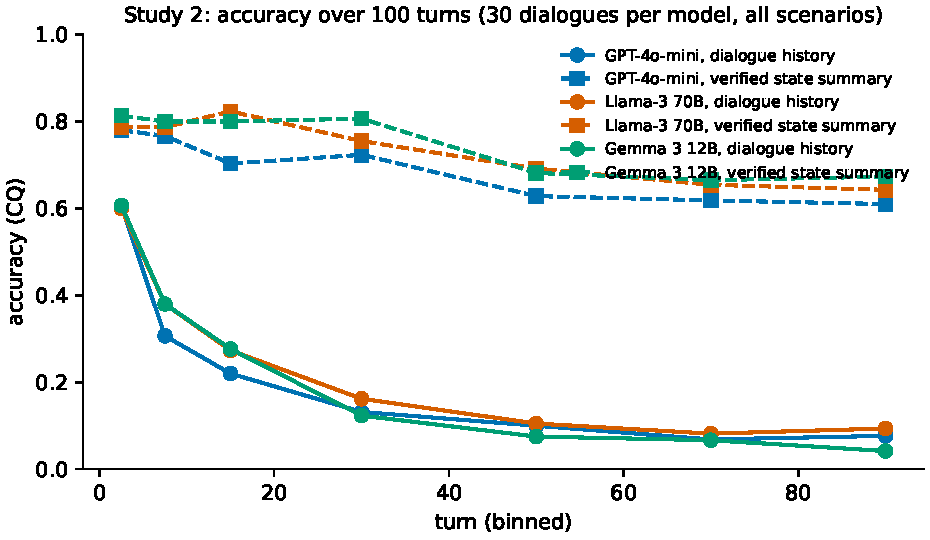
\includegraphics[width=0.85\linewidth]{study2_accuracy_over_turns.pdf}
\caption{Study 2 accuracy over 100 turns, pooled over the five scenarios.
Solid lines show the dialogue history; dashed lines show the verified state
summary. The control's gradual decline reflects the scheduled difficulty
increases in S1--S3.}
\label{fig:s2}
\end{figure}

\paragraph{A verified state summary preserves accuracy.}
GPT-4o-mini answered the same questions from the verified state summary with an
accuracy of \cdrGptCtrlLate{} over turns 21--100, against \cdrGptLate{} under
dialogue history. Under the summary its accuracy also followed the scheduled
difficulty regimes.

The frozen completion test confirmed this mitigation in the two-model family.
Over turns 1--100, the per-dialogue control-minus-history gap was
\cdrLlamaControlGap{} for Llama-3 70B (95\% bootstrap CI
[\cdrLlamaControlCiLo{}, \cdrLlamaControlCiHi{}]) and
\cdrGemmaControlGap{} for Gemma 3 12B (95\% CI
[\cdrGemmaControlCiLo{}, \cdrGemmaControlCiHi{}]); both one-sided sign-flip
tests remained significant after Holm correction
($p=\cdrLlamaControlHolmP{}$ and $p=\cdrGemmaControlHolmP{}$, respectively;
30 paired dialogues per model). The secondary turns 21--100 gaps were
\cdrLlamaControlLateGap{} and \cdrGemmaControlLateGap{}. Table~\ref{tab:s2control}
reports the frozen primary family, including the previously observed
GPT-4o-mini estimate outside that family.

\begin{table}[t]
\centering
\caption{Frozen H-C1: per-dialogue mean accuracy difference between verified
state summary and dialogue history over turns 1--100. The GPT-4o-mini result
was already observed and was excluded from the Holm family.}
\label{tab:s2control}
\small
\begin{tabular}{lcccc}
\toprule
Model & Mean gap & 95\% bootstrap CI & Holm $p$ & Dialogues\\
\midrule
\inputtable{generated/table_cdr_control_completion.tex}
\bottomrule
\end{tabular}
\end{table}

Because the dialogue arm was already near the floor, the frozen pre/post
change-point contrasts of the dialogue arm were dominated by the background
collapse. We therefore do not interpret them as task-drift effects (see the
supplement).
